\documentclass[compress]{beamer}
\usepackage{ifthen,verbatim}

\title{Correcting a mistake in the alignment procedure \\ unveiled by the CSA07 alignment exercise}
\author{Jim Pivarski, Alexei Safonov}
\institute{Texas A\&M University}
\date{ 8 November, 2007}

\newcommand{\isnote}{}
\xdefinecolor{lightyellow}{rgb}{1.,1.,0.25}
\xdefinecolor{darkblue}{rgb}{0.1,0.1,0.7}

%% Uncomment this to get annotations
%% \def\notes{\addtocounter{page}{-1}
%%            \renewcommand{\isnote}{*}
%% 	   \beamertemplateshadingbackground{lightyellow}{white}
%%            \begin{frame}
%%            \frametitle{Notes for the previous page (page \insertpagenumber)}
%%            \itemize}
%% \def\endnotes{\enditemize
%% 	      \end{frame}
%%               \beamertemplateshadingbackground{white}{white}
%%               \renewcommand{\isnote}{}}

%% Uncomment this to not get annotations
\def\notes{\comment}
\def\endnotes{\endcomment}

\setbeamertemplate{navigation symbols}{}
\setbeamertemplate{headline}{\includegraphics[height=1 cm]{../cmslogo} \hspace{0.1 cm} \includegraphics[height=1 cm]{../tamulogo} \hfill
\begin{minipage}{5.5 cm}
\vspace{-0.75 cm} \small
\begin{center}
\ifthenelse{\equal{\insertpagenumber}{1}}{}{\textcolor{blue}{\insertsection}}
\end{center}
\end{minipage} \hfill
\begin{minipage}{4.5 cm}
\vspace{-0.75 cm} \small
\begin{flushright}
\ifthenelse{\equal{\insertpagenumber}{1}}{}{Jim Pivarski \hspace{0.5 cm} \insertpagenumber\isnote/\pageref{numpages}}
\end{flushright}
\end{minipage}\mbox{\hspace{0.2 cm}}}

\begin{document}
\frame{\titlepage}

%% \begin{notes}
%% \item This is the annotated version of my talk.
%% \item If you want the version that I am presenting, download the one
%% labeled ``slides'' on Indico (or just ignore these yellow pages).
%% \item The annotated version is provided for extra detail and a written
%% record of comments that I intend to make orally.
%% \item Yellow notes refer to the content on the {\it previous} page.
%% \item All other slides are identical for the two versions.
%% \end{notes}

\section*{Mistake in alignment procedure}

\begin{frame}
\frametitle{The story in brief}
\begin{itemize}\setlength{\itemsep}{0.25 cm}
\item I have been presenting alignment results for some time now
\item CSA07 was supposed to be inconsequentially different (details next slide)
\item We did not reproduce old alignment in CSA: 100 microns resolution $\to$ 1 mm!
\item Extensive diagnostics ensued\ldots
\item Conclusion: the old alignment procedure is at fault, previous results were too optimistic
\item We corrected our procedure and are now re-optimizing it
\item Old questions must be reopened, systematics studies repeated
\end{itemize}
\end{frame}

\begin{frame}
\frametitle{Differences between CSA07 and previous studies}
\begin{itemize}\setlength{\itemsep}{0.5 cm}
\item \textcolor{darkblue}{Miscalibrated hits}

\vspace{0.25 cm}
Miscalibration effect studied in isolation: too small to account for differences

\item \textcolor{darkblue}{CMSSW version 1\_6\_4 instead of 1\_5\_4}

\vspace{0.25 cm}
Reconstructed and aligned one sample in all 4 combinations of releases: no errors

\item \textcolor{darkblue}{Tracks fit with misalignments}

\vspace{0.25 cm}
Reconstructed with and without misalignments at each stage of
reconstruction: the problem is in track-fitting with misalignments
\end{itemize}
\end{frame}

\begin{frame}
\frametitle{Background: misalignments in alignment simulations}

\begin{itemize}
\item \textcolor{darkblue}{In the detector simulation:} defines the ``true'' geometry, the objective of
alignment, in the same way as data.  Not yet possible in CMSSW.

\item \textcolor{darkblue}{In track reconstruction:} weak effect on the choice of hits
associated with tracks (roads are wide compared to misalignments),
strong effect on the fitted track, but we refit the track in alignment

\item \textcolor{darkblue}{In the alignment process:} strong effect on
the refitted tracks in the first iteration
\end{itemize}

\vspace{0.1 cm}
We have always misaligned in the alignment process; in CSA07, we
also misaligned the initial track reconstruction (RECO job)

\vspace{0.2 cm}
Lost $\sim$0.5 hits per track due to RECO misalignment: cannot account for 10$\times$ degradation in alignment!
\end{frame}

\begin{frame}
\frametitle{How globalMuon alignment is {\it supposed} to work}

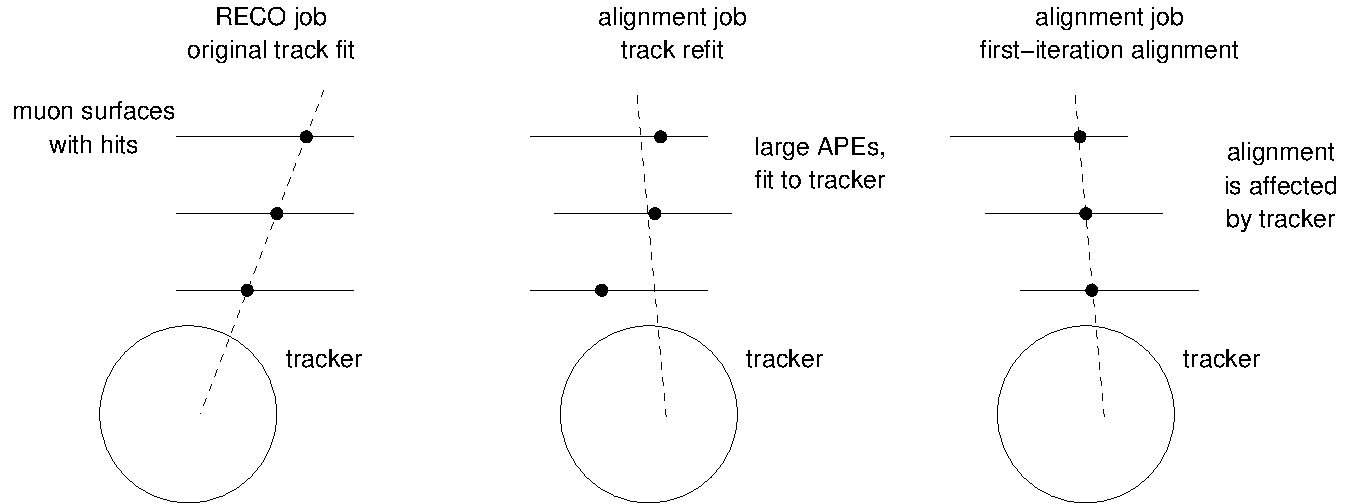
\includegraphics[width=\linewidth]{premistake.pdf}

\vfill Geometry used in RECO is irrelevant because tracks are refit.
Muon hits are deweighted with large Alignment Parameter Errors (APEs) to
effectively fit to tracker and extrapolate to muon system
\end{frame}

\begin{frame}
\frametitle{Mistake in the old procedure: outside-in fits}

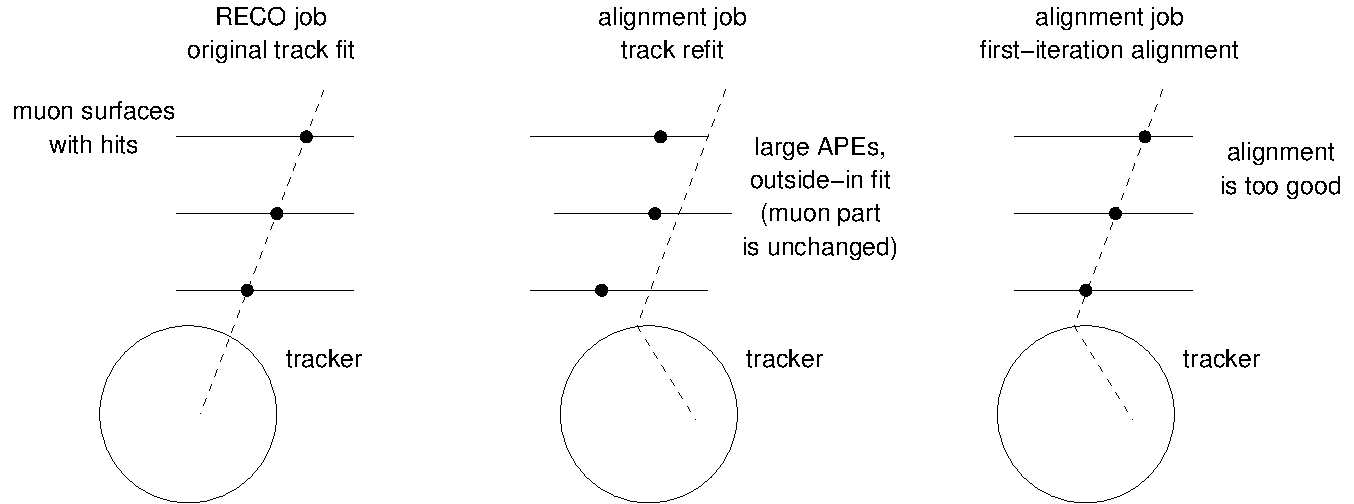
\includegraphics[width=\linewidth]{mistake.pdf}

\vfill Ideal RECO geometry creates ideally-fitted tracks.  Refitting
starts from the outside and works inward, {\it causing minimal changes
to track parameters} because of the large APEs.

\vfill Alignment output was too good because information about the
ideal geometry was encoded in the unchanged part of the track
\end{frame}

\begin{frame}
\frametitle{How we found it with CSA07}

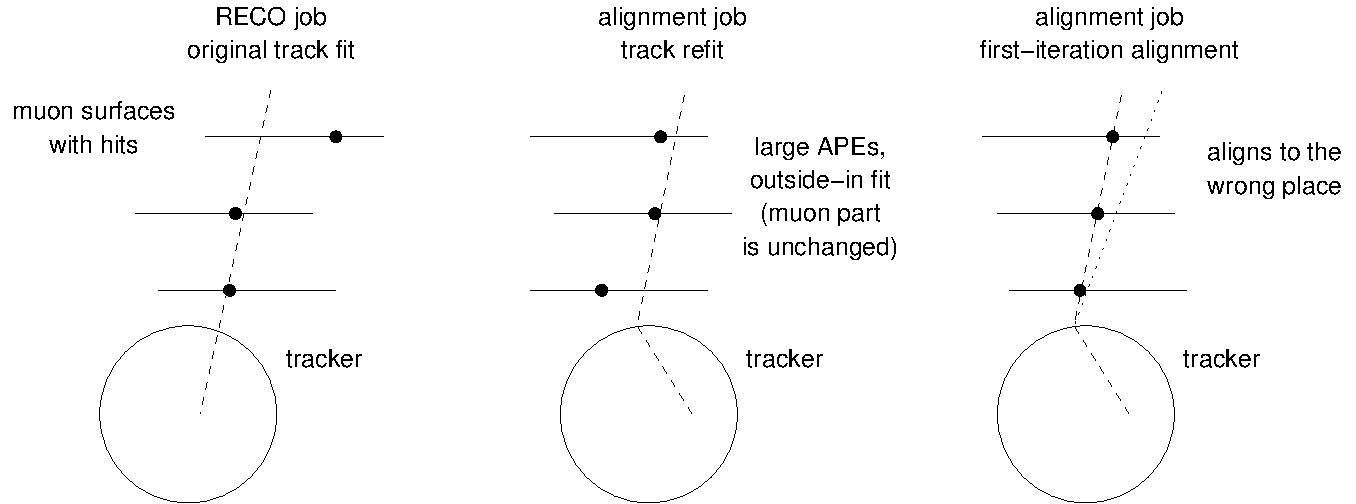
\includegraphics[width=\linewidth]{mistake2.pdf}

\vfill CSA07 event samples are misaligned at the RECO level, so we get
a non-ideal track seed.  The muon part of the track is again not
changed, so we incorrectly align to whatever was used in RECO.

\vfill Hence, difference from ideal is large.
\end{frame}

\begin{frame}
\frametitle{Lessons}

\vspace{-0.25 cm}
\begin{enumerate}
\item In a globalMuon alignment (extrapolating from tracker to muon system),
always use an inside-out fit!
\item In a standAloneMuon alignment, don't make APEs too large!
\item Corrected simulation results $\approx$ muon alignment scenarios
\end{enumerate}

\vfill
\hspace{-0.83 cm} \textcolor{darkblue}{\Large What to do about it} \hfill (\textcolor{darkblue}{blue} is new, black is an update)
\begin{itemize}
\item \textcolor{darkblue}{Optimize a new procedure using inside-out fits}
\item \textcolor{darkblue}{Choose a $p_T$ cut in a generic sample} \\ \textcolor{darkblue}{(revisit low momentum now that we need statistics)}
\item CSA with 10 and 100 pb$^{-1}$: make baseline alignment scenarios
\item Systematics studies: tracker misalignment, miscalibration,
\textcolor{darkblue}{material/$\vec{B}(\vec{x})$ dependence}
\item Study performance in standAlone muon $Z$, globalMuon $Z'$/Drell-Yan
\end{itemize}
\end{frame}

\section*{New alignment procedure}

\begin{frame}
\begin{center}
\Huge \textcolor{blue}{Optimizing a new alignment procedure}
\end{center}
\end{frame}

\begin{frame}
\frametitle{Alignment with inside-out fits}

100k events (25 pb$^{-1}$), 8 mm APEs, 3 iterations

\begin{center}
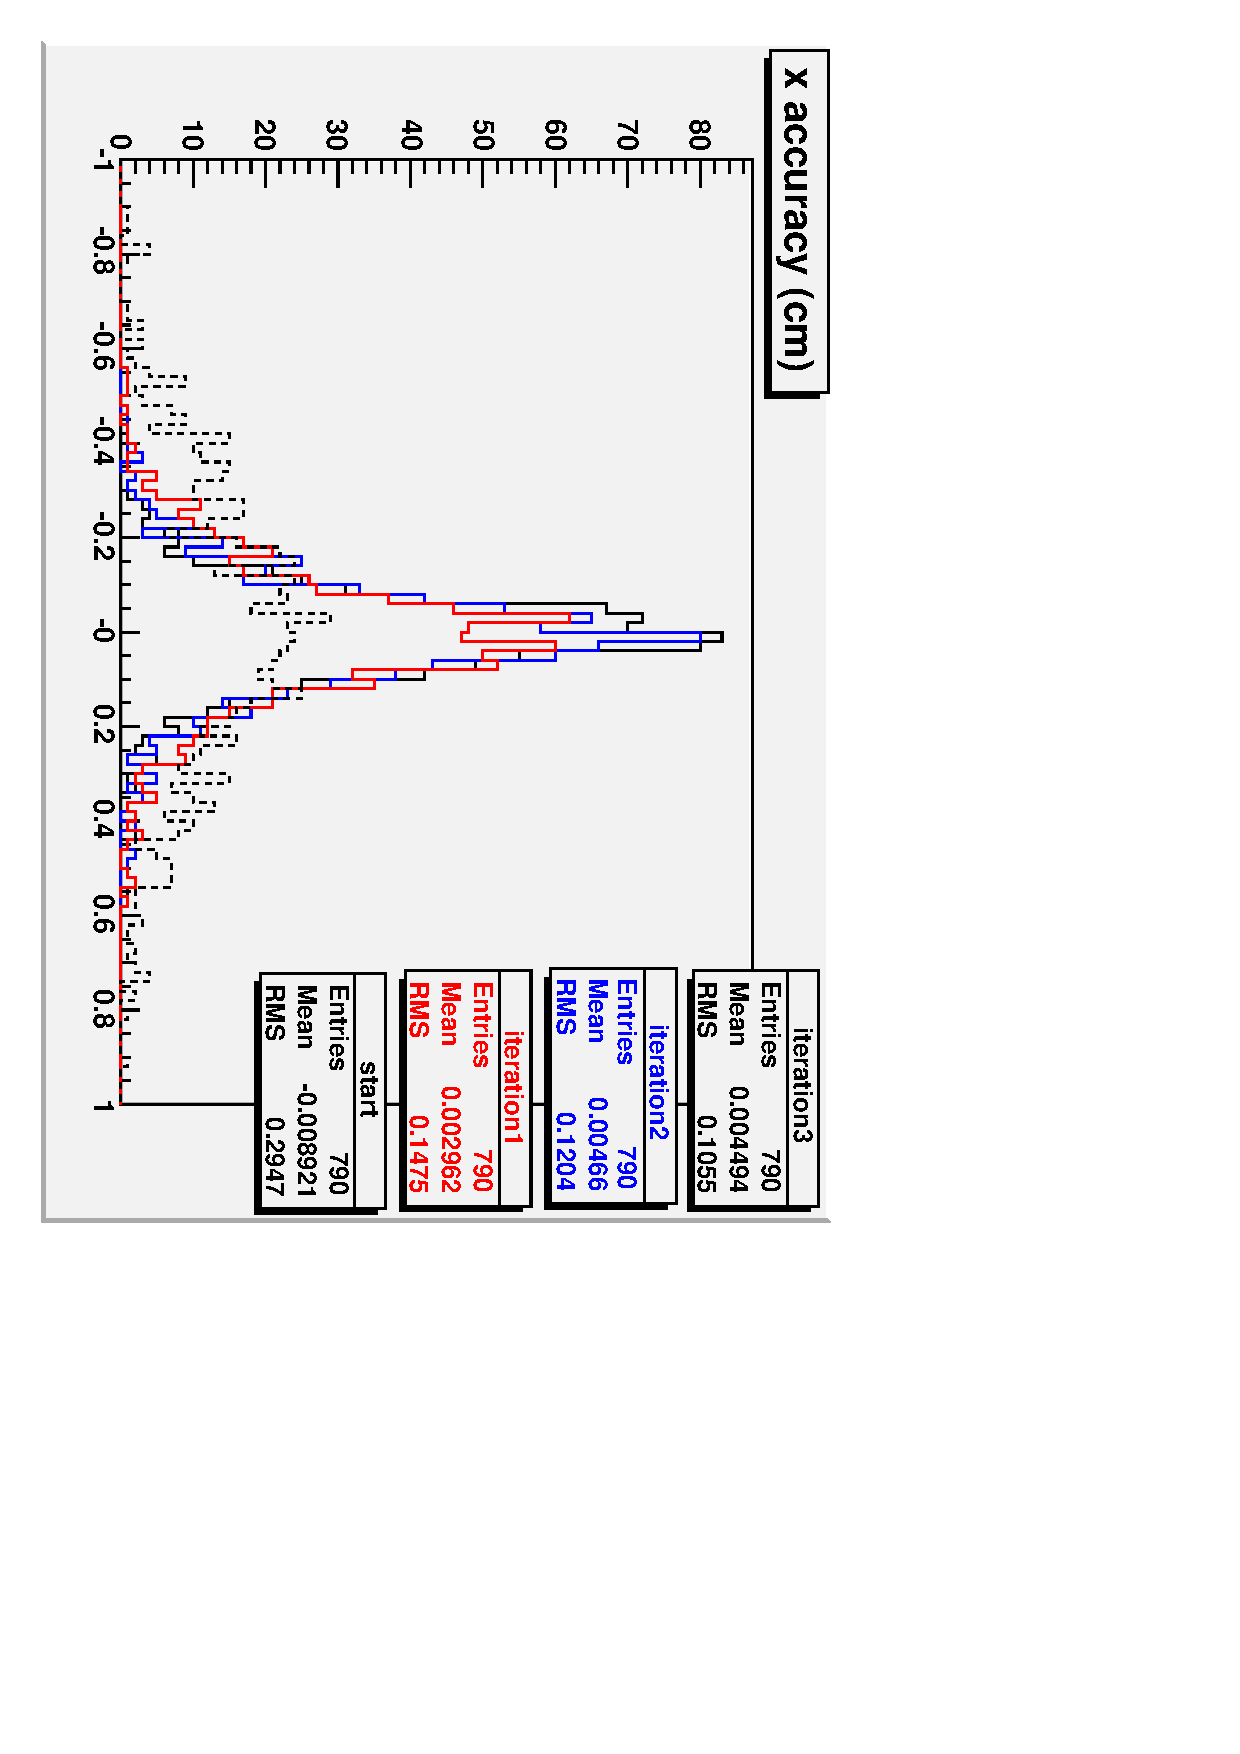
\includegraphics[height=0.6\linewidth, angle=90]{xaccuracy_3iters.pdf}
\end{center}

\vspace{-0.25 cm}
\hspace{-0.5 cm} \begin{minipage}{\linewidth}
\begin{tabular}{c c c c c}
& 1 & 2 & 3 & 4 \\\hline
Muon barrel stations & 490~$\mu$m & 680~$\mu$m & 960~$\mu$m & 1.4~mm \\
Muon endcap ME$x$/1 stations & 510~$\mu$m & 670~$\mu$m & 980~$\mu$m & 1.1~mm\\
Muon endcap ME$x$/2 stations & 830~$\mu$m & 1.2~mm & 1.5~mm & \\
\end{tabular}
\end{minipage}
\end{frame}

\begin{frame}
\frametitle{Problem: scattering in material is cumulative}

\hspace{-0.83 cm} \textcolor{darkblue}{\Large Solution: minimize extrapolation by aligning in stages}
\begin{enumerate}
\item Align station 1 only with loose APEs
\item Align station 2 with tight APEs on 1, loose on the rest
\item \ldots
\end{enumerate}

\vfill Test-scenarios (local $x$ only, 10 pb$^{-1}$) 
\begin{itemize}
\item 3~mm Gaussian misalignment for unaligned chambers
\item 1~cm coherent misalignment for chambers under study
\item $\sqrt{N}\times$500~$\mu$m Gaussian residual misalignment for
aligned chambers ($N$ is the station number)
\item Vary ``loose'' APEs on chambers under study 0.7--5~cm
\item Vary ``loose'' APEs on outer chambers 0.7--5~cm
\end{itemize}
\end{frame}

\begin{frame}
\frametitle{Innermost barrel station (MB1)}
\begin{center}
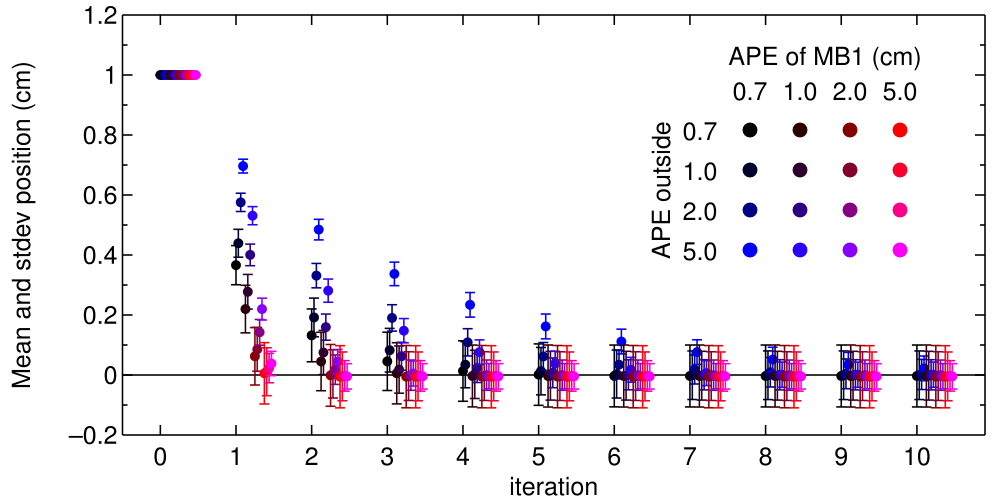
\includegraphics[width=\linewidth]{mb1_meanstdev.png}
\end{center}

\vspace{-0.5 cm}
\begin{itemize}
\item Large APE on MB1 improves convergence of mean (accuracy)
\item Large APE on MB2, MB3, MB4 reduces stdev (precision)
\item Dropping MB2, MB3, MB4 from fit (infinite APE) is worse
\end{itemize}
\end{frame}

\begin{frame}
\frametitle{Innermost endcap station (ME1/1)}
\begin{center}
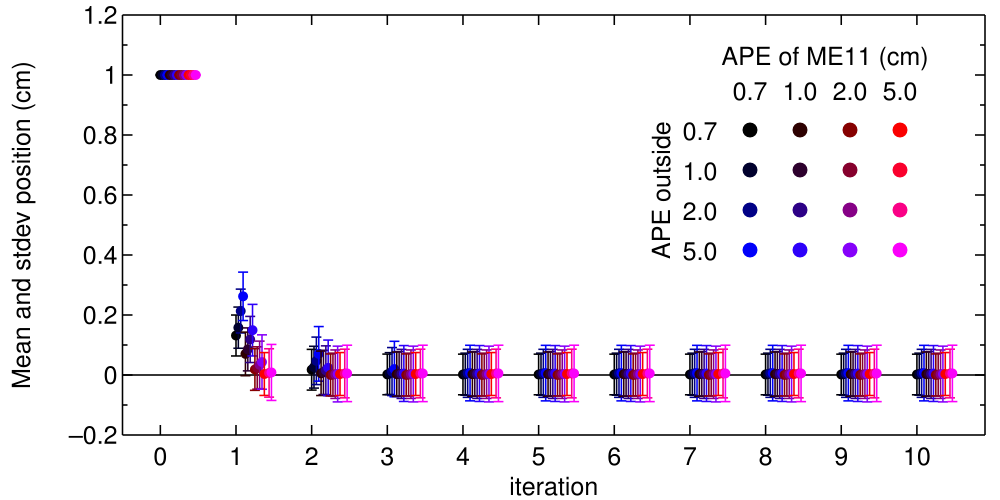
\includegraphics[width=\linewidth]{me11_meanstdev.png}
\end{center}

\vspace{-0.5 cm}
\begin{itemize}
\item All cases converge quickly
\item All stdevs are large (680~$\mu$m)
\end{itemize}
\end{frame}

\begin{frame}
\frametitle{All the rest (discussion on next slide)}
\begin{tabular}{p{0.3\linewidth} p{0.3\linewidth} p{0.3\linewidth}}
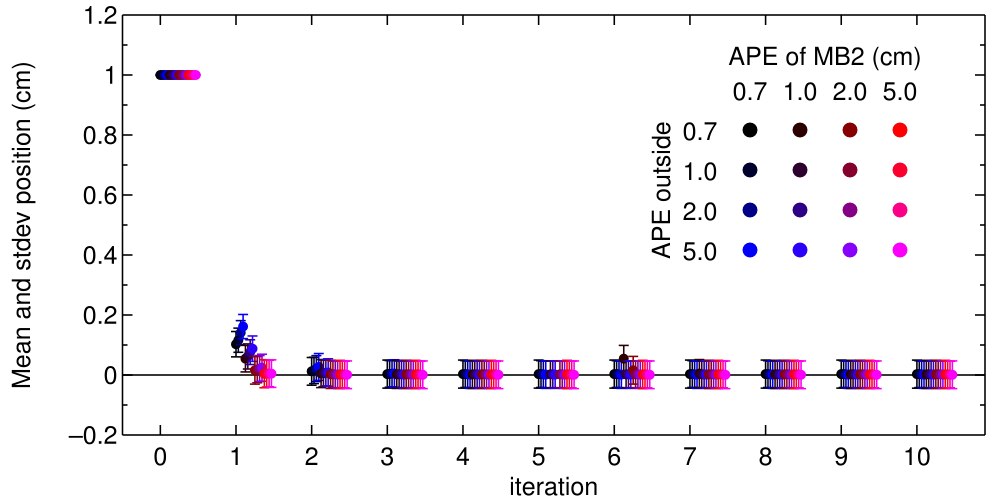
\includegraphics[width=\linewidth]{mb2_meanstdev.png} &
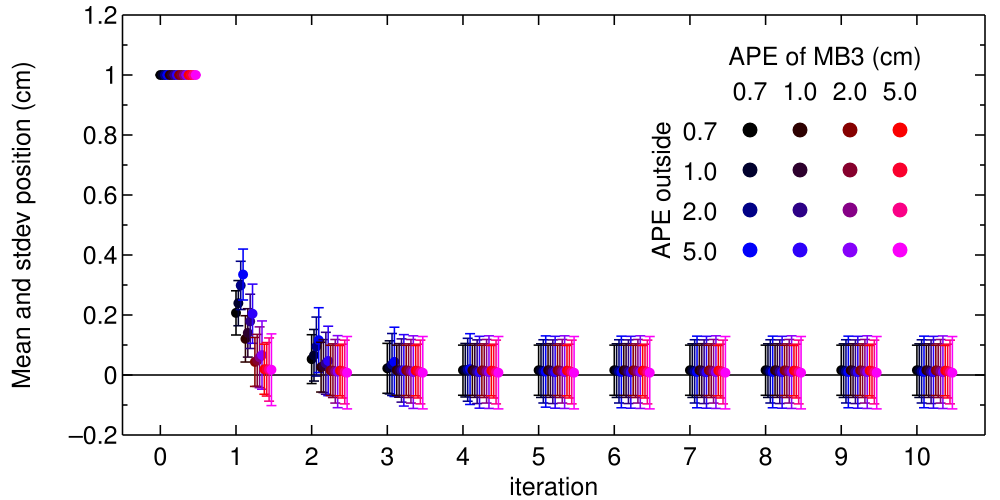
\includegraphics[width=\linewidth]{mb3_meanstdev.png} &
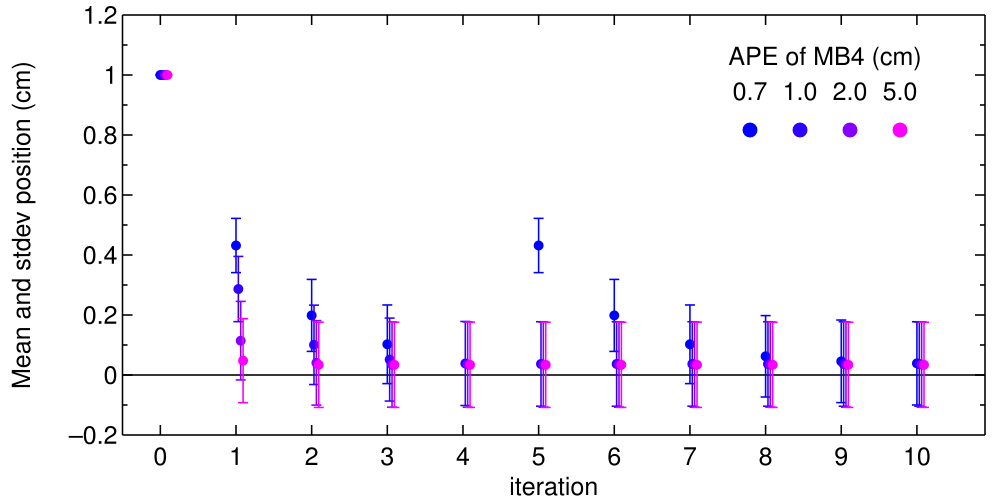
\includegraphics[width=\linewidth]{mb4_meanstdev.png} \\
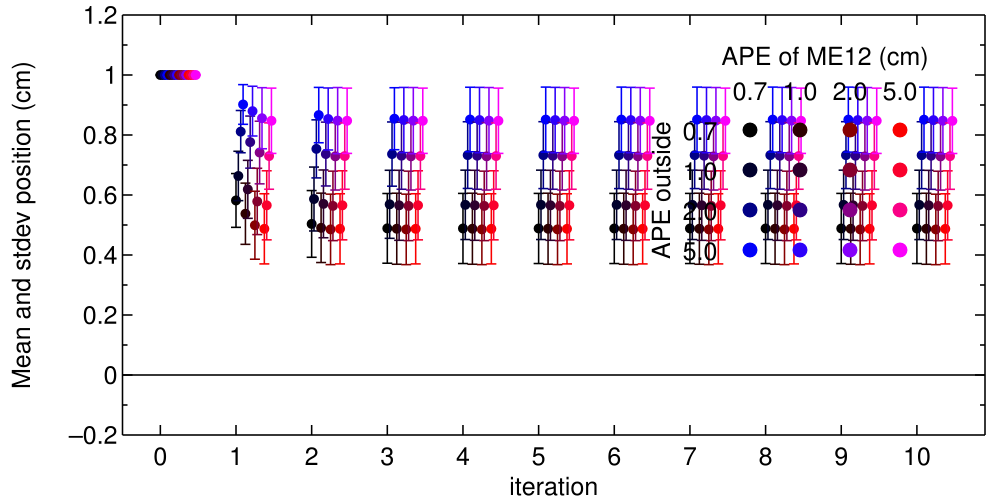
\includegraphics[width=\linewidth]{me12_meanstdev.png} &
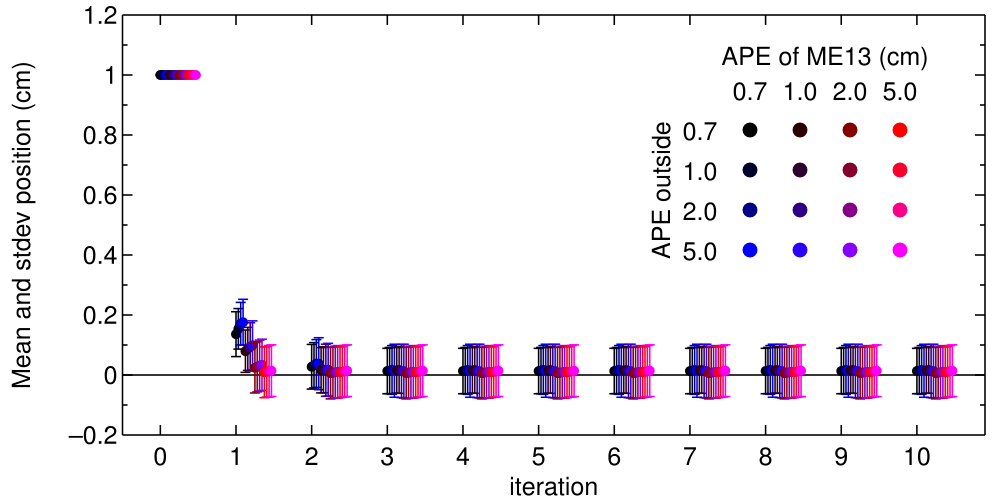
\includegraphics[width=\linewidth]{me13_meanstdev.png} & \\
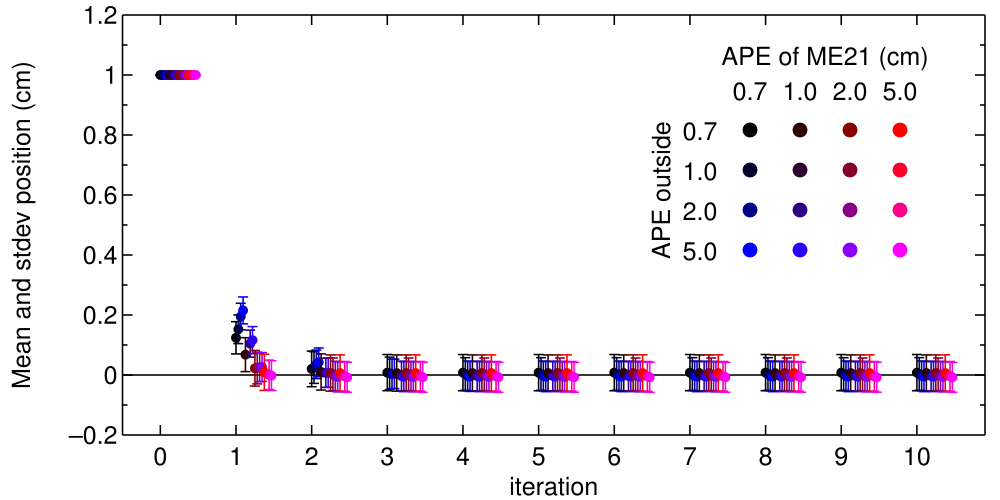
\includegraphics[width=\linewidth]{me21_meanstdev.png} &
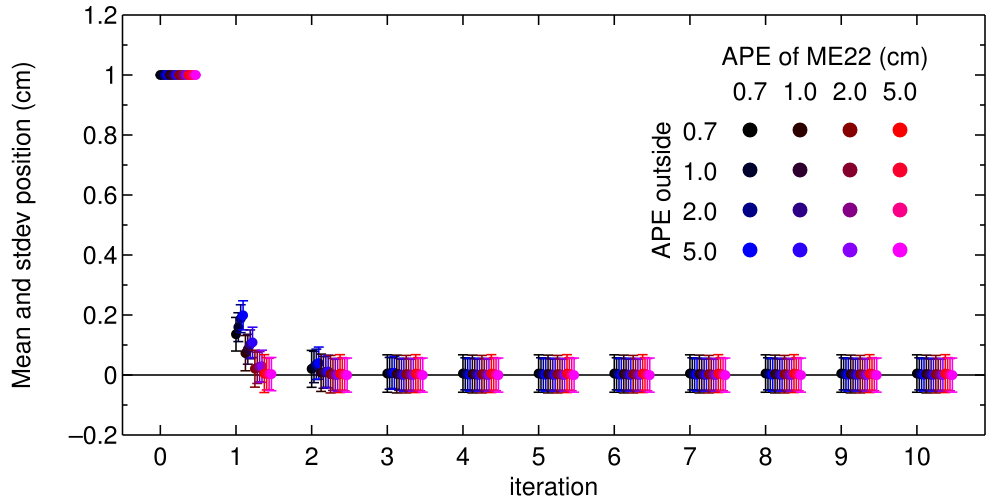
\includegraphics[width=\linewidth]{me22_meanstdev.png} & \\
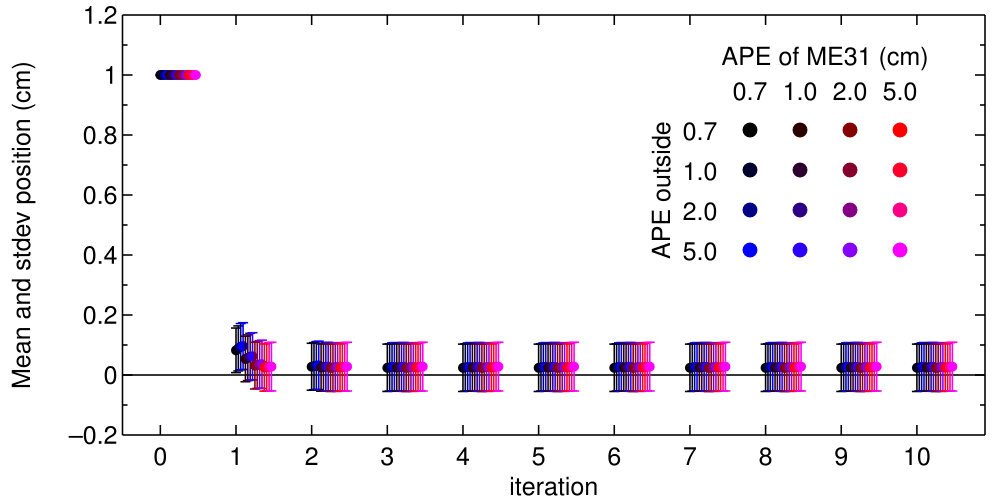
\includegraphics[width=\linewidth]{me31_meanstdev.png} &
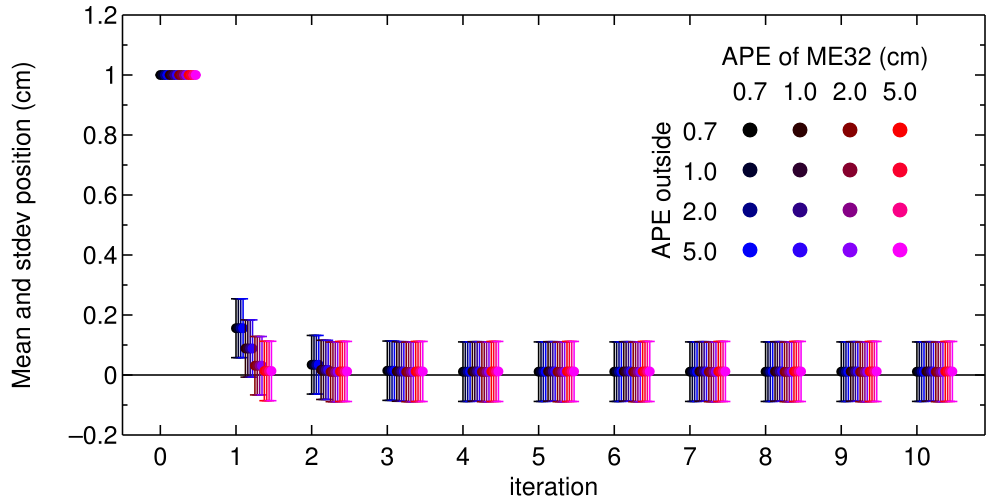
\includegraphics[width=\linewidth]{me32_meanstdev.png} & 
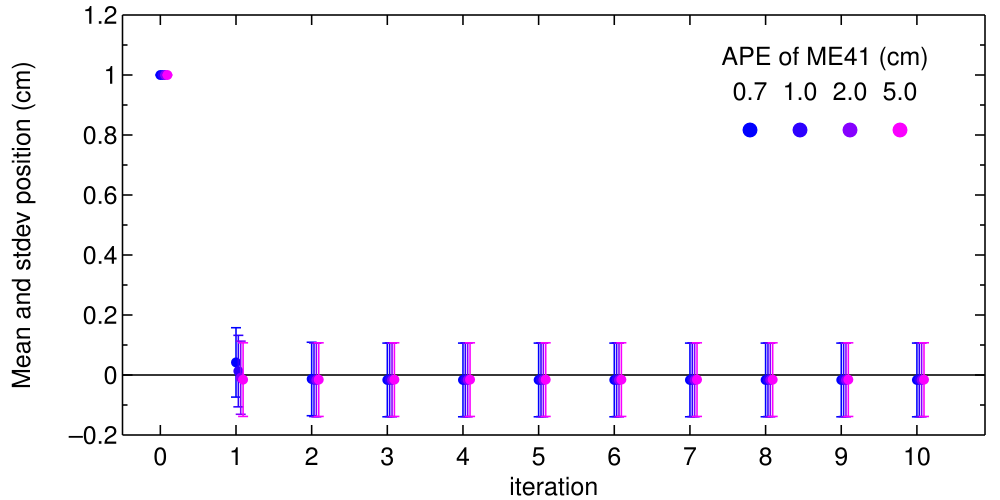
\includegraphics[width=\linewidth]{me41_meanstdev.png}
\end{tabular}
\end{frame}

\begin{frame}
\begin{itemize}
\item ME1/2 did not converge!  Loosen APEs: 5, 7, 10, 15~cm
\item Why ME1/2?  What's special about it?  The solenoid?
\end{itemize}

\vspace{-0.25 cm}
\begin{center}
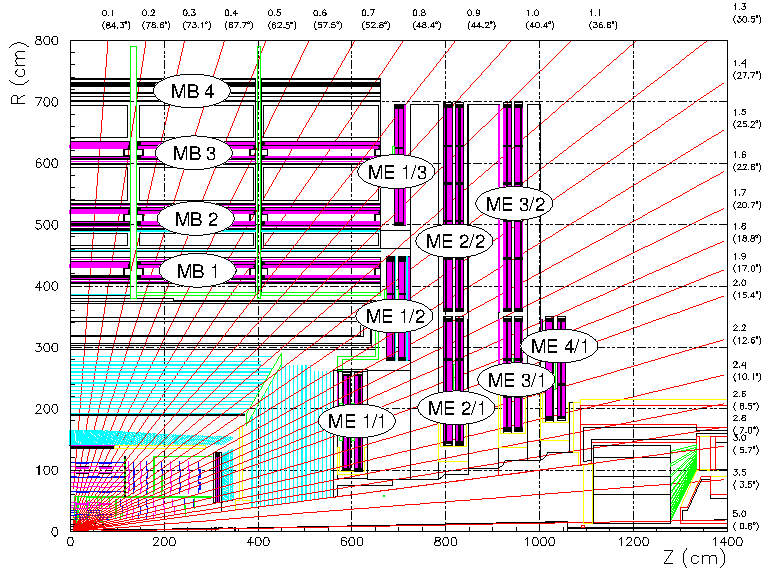
\includegraphics[width=0.6\linewidth]{muon_system_labeled.pdf}
\end{center}

\vspace{-0.5 cm}
\begin{itemize}
\item Only in MB1 do we see a range of convergence speeds (parameters
were chosen using MB1 as a test-case)
\item For the rest (excluding ME1/2), tighten APEs to get more
precision at the expense of convergence: 0.05, 0.1, 0.2, 0.5~cm
\end{itemize}
\end{frame}

\begin{frame}
\frametitle{Current status}

\begin{itemize}\setlength{\itemsep}{0.25 cm}
\item Station-by-station results are about a factor of 2 better
than all-at-once method (taking $\sqrt{\mbox{25 pb$^{-1}$}/\mbox{10
pb$^{-1}$}}$ into account)
\item But they still show a strong dependence on cumulative
propagation (either material or cumulative error)
\end{itemize}

\vspace{0.25 cm}
\hspace{-0.5 cm} \begin{minipage}{\linewidth}
\begin{tabular}{c c c c c}
& 1 & 2 & 3 & 4 \\\hline
Muon barrel stations & 420~$\mu$m & 440~$\mu$m & 850~$\mu$m & 1.5~mm \\
Muon endcap ME$x$/1 stations & 680~$\mu$m & 490~$\mu$m & 822~$\mu$m & 1.2~mm\\
Muon endcap ME$x$/2 stations & 770~$\mu$m & 520~$\mu$m & 1.0~mm & \\
\end{tabular}
\end{minipage}

\vspace{0.25 cm}
\begin{itemize}\setlength{\itemsep}{0.25 cm}
\item Standard 10~pb$^{-1}$ scenario has 500~$\mu$m misalignments

\item Relative alignments are much more precise: if we had no
uncertainty in MB1, MB2 would have 70~$\mu$m resolution; worst {\it
relative} case is 270~$\mu$m (ME1/1 $\to$ ME2/1)
\end{itemize}

\vfill
\mbox{ }
\end{frame}

\begin{frame}
\frametitle{Next steps}
\begin{enumerate}\setlength{\itemsep}{0.5 cm}
\item Optimize globalMuon and/or standAlone muon procedure
\item Scale best case up to 100~pb$^{-1}$
\item Do a full alignment exercise with $Z\to\mu\mu$ (CSA07-1)
\item Apply alignment results to physics ($Z$, $Z'$, Drell-Yan)
\item Explore low-momentum muons ($Z$$+$$W$$+$QCD-mu: CSA07-2)
\item Re-do systematics studies, including material $\rho(\vec{x})$ and
$\vec{B}(\vec{x})$ (which I now know how to do)
\end{enumerate}
\label{numpages}
\end{frame}

\end{document}
